% -------------------------------------------------------------------------------- %

\begin{exercise}

Sei $I \subseteq \R$ ein offenes Intervall um den Nullpunkt und $g, f \in C^1(\R)$.
Betrachten Sie das Cauchyproblem

\begin{align*}
    u_t + g(u) u_x = 0,
    \quad
    u(0, x) = f(x)
\end{align*}

für $(t, x) \in I \times \R$.

\begin{enumerate}[label = (\roman*)]

    \item Bestimmen Sie die Charakteristiken und überprüfen Sie, ob die Voraussetzungen für den Existenzsatz 2.3 erfüllt sind.

    \item Bestimmen Sie eine Lösung für die Burgers-Gleichung

    \begin{align*}
        u_t + u u_x = 0,
        \quad
        (t, x) \in \R^2
    \end{align*}

    mit den Anfangsdaten $u(0, x) = -x$ und geben Sie den Definitionsbereich der Lösung an.
    Skizzieren Sie die Charakteristiken und die Lösung zu verschiedenen Zeitpunkten.

\end{enumerate}

\end{exercise}

% -------------------------------------------------------------------------------- %

\begin{solution}

\phantom{}

\begin{enumerate}[label = (\roman*)]

	\item Unsere Differentialgleichung hat die Form

	\begin{gather*}
		\overline{t}(y) = 0,
		\overline{x}(y) = y,
		\overline{u}(y) = f(y), \\
		\Gamma = \Bbraces
		{
			(\overline{t}(y), \overline{x}(y)):
			y \in \R
		},
		\quad
		S = \Bbraces
		{
			(\overline{t}(y), \overline{x}(y), \overline{u}(y)):
			y \in \R
		}, \\
		a(t, x, u) u_t + b(t, x, u)u_x = c(t, x, u), \\
		a(t,x,u) = 1, \quad b(t,x,u) = g(u), \quad c(t,x,u) = 0.
	\end{gather*}

	Wir haben gelernt wie man so eine Differentialgleichung mit der Charakteristikenmethode löst. Dafür lösen wir als erstes das System an Differentialgleichungen

	\begin{align*}
		\pderivative[][t]{s} = a(t,x,u) = 1, \quad \pderivative[][x]{s} = b(t,x,u) = g(u), \quad \pderivative[][u]{s} = c(t,x,u) = 0.
	\end{align*}

	Aus der Nebenbedingung ergeben sich für die Lösungen noch zusätzlich die Bedingungen

	\begin{align*}
		t(0, y) = \overline{t}(y) = 0,
		\quad
		x(0, y) = \overline{x}(y) = y,
		\quad,
		u(0, y) = \overline{u}(y) = f(y).
	\end{align*}

	Die erste und letzte ODE löst man mit Integration nach $s$.
	Die Integrationskonstante ergibt sich aus dem Anfangswert.

	\begin{align*}
		\implies
		t(s,y) = s,
		\quad
		u(s,y) = f(y)
	\end{align*}

	Damit, und einer weiteren Integration (einer $s$-Konstanten), bekommt man die Lösung der zweiten ODE.

	\begin{align*}
		\pderivative[][x]{s}(s,y) = g(u(s,y)) = g(f(y))
		\implies
		x(s, y) = s \cdot g(f(y)) + y.
	\end{align*}

	Für festes $y$ ist also eine Charakteristik gegeben durch

	\begin{align*}
		(t^{(y)}(s), x^{(y)}(s), u^{(y)}(s))
		=
		(s, s \cdot g(f(y)) + y, f(y)).
	\end{align*}

	Sind die Voraussetzungen von Satz 2.3 erfüllt? Wir rechnen nach.

	\begin{align*}
		\det \pderivative[][(t,x)]{(s,y)} = \det
		\begin{pmatrix}
			t_s(0,y) & t_y(0,y) \\
			x_s(0,y) & x_y(0,y)
		\end{pmatrix}
		=
		\det
		\begin{pmatrix}
			a(t, x, u) & \overline{t}_y(y) \\
			b(t, x, u) & \overline{x}_y(y)
		\end{pmatrix}
		=
		\det
		\begin{pmatrix}
			1 & 0 \\
			g(f(y)) & 1
		\end{pmatrix}
		= 1 \neq 0
	\end{align*}

	Und wir sehen, dass die Voraussetzungen des Satzes erfüllt sind, es gibt also lokal eine Lösung.

	\item Nun haben wir es mit einem Spezialfall des bisher Betrachteten zu tun, nämlich mit $g(u) = u$ und $f(x) = -x$. Wir nützen die Ergebnisse vom vorigen Teil und erhalten

	\begin{align*}
		t(s,y) & = s, \\
		x(s,y) & = s \cdot g(f(y)) + y = s \cdot g(-y) + y = -sy + y = y(1 - s), \\
		u(s,y) & = f(y) = -y
	\end{align*}

	Es ergibt sich also

	\begin{align*}
		t = s
		& \iff
		s = t \\
		x = y(1 - s) = y(1 - t)
		& \iff
		y = \frac{x}{1 - t}
	\end{align*}

	und damit als Lösung

	\begin{align*}
		u(t,x) = u(s(t,x), y(t,x)) = y(t,x) = \frac{x}{t - 1},
	\end{align*}

	eine auf $(\R \setminus \Bbraces{1}) \times \R$ definierte Funktion.
	Plots dazu findet man in den Abbildungen \ref{fig:lsg_u_char} und \ref{fig:lsg_u_graph}.

	\begin{figure}[h!]
		\centering
		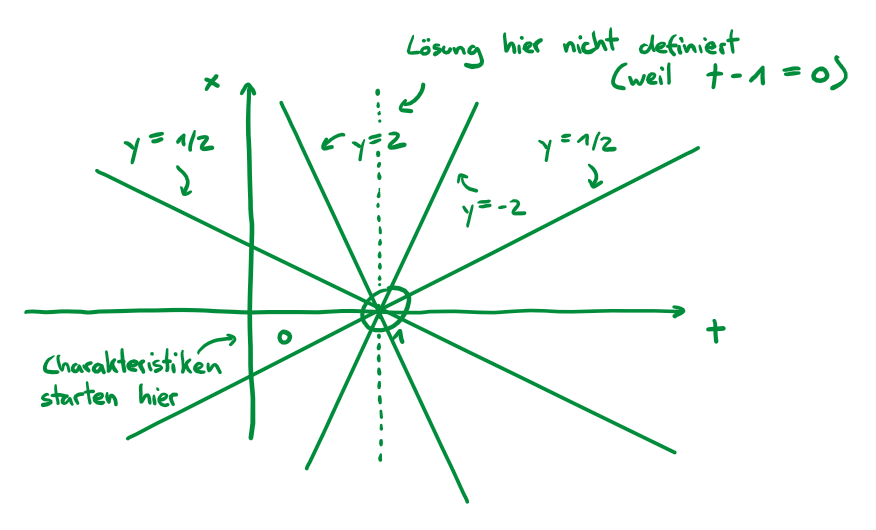
\includegraphics[width = 0.75 \textwidth]{2-3-1.png}
		\caption{Charakteristiken von $u$ im $\R^2$}
		\label{fig:lsg_u_char}
	\end{figure}

	\begin{figure}[h!]
		\centering
		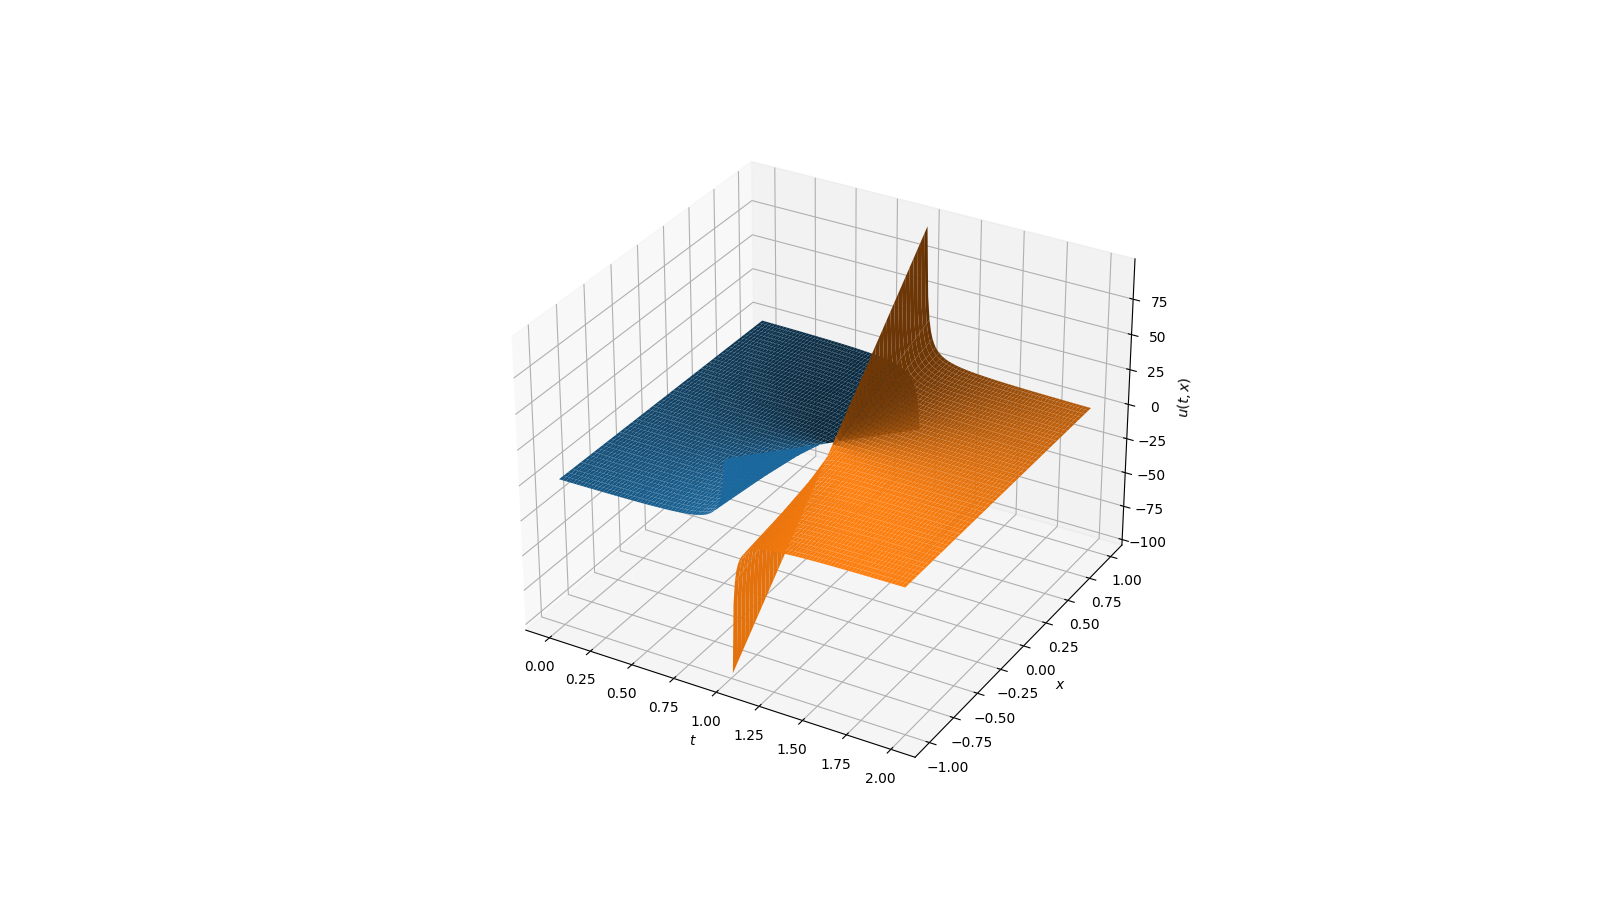
\includegraphics[width = \textwidth]{2-3-2.png}
		\caption{Graph von $u$ im $\R^3$}
		\label{fig:lsg_u_graph}
	\end{figure}
\end{enumerate}

\end{solution}

% -------------------------------------------------------------------------------- %
